This section documents the validations of the Matrix Element method by measuring the 
$\WZ/ZZ$ cross-sections. This part of the analysis is performed with the 
Spring11 MC corresponding to the EPS selections. 

We validate performance of our implementation of the Matrix Element technique by simultaneously measuring
$WZ$ and $ZZ$ cross-section in the zero jet bin. 
%in events with two-charged leptons and missing transverse energy.
After the preselection cuts, the only relevant background in the measurement is non-resonant $WW$ production.
Therefore, the main challenge is to discriminate $ZZ$ and $WZ$ events from $WW$.

In order to achieve this, we construct new Likelihood $LR_{ZZ+WZ}$, defined as:
\begin{equation}
\label{eqn:LRZZ}
LR_{ZZ+WZ} = \frac { P_{ZZ}+P_{WZ}} { P_{ZZ} + P_{WZ} + P_{WW} },
\end{equation}
where $P_{WZ}$ is evaluated with the assumption that two charged leptons originated from a $Z$-boson, while 
$W$ leptonically but the lepton was not reconstructed. Distribution of LR$_{ZZ+WZ}$ for data and predicted 
backgrounds and signal is shown in figure \ref{fig:lrzz}. One can see that shape of the  distribution in data is well 
modeled.

%%%%%%%%%%%%%%%%%%%%%%%%%%%%%%
\begin{figure}[!htbp]
\begin{center}
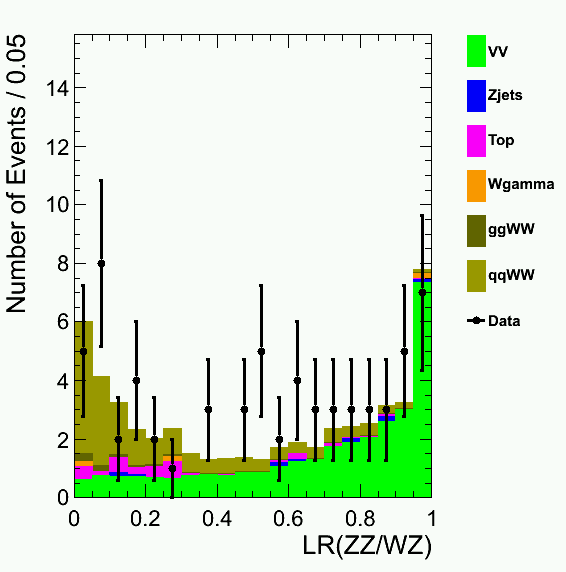
\includegraphics[width=0.5\textwidth]{figures/LRZZ.png}
\caption{$LR_{ZZ+WZ}$ in 1092 pb$^{-1}$ of data compared to expected backgrounds and $ZZ+WZ$ signal.}
\label{fig:lrzz}
\end{center}
\end{figure}
%%%%%%%%%%%%%%%%%%%%%%%%%%%%%%

Precise measurement of the cross-section requires clean sample of signal events. We, therefore, further select events
that pass $LR_{ZZ+WZ}>0.75$ requirement. Expected yields for each process as well as observed data count is shown in table \ref{tab:ZZWZselection}.

\begin{table}[!ht]
  \begin{center}
 {\scriptsize
  \begin{tabular} {|c|c|}
 \hline
  Process & Events \\
  \hline
  \hline
  $qq \rightarrow WW$   &  1.4 $\pm$   0.1 \\
  $gg \rightarrow WW$   &  0.1 $\pm$   0.01 \\
  $tt + tw$             &  0.15 $\pm$  0.05 \\
  $Z  + jets$           &  0.43 $\pm$  0.2 \\
  $W  + \gamma$          &  0.17 $\pm$  0.17 \\
  \hline
  Total Background      &  2.25 $\pm$  0.53 \\
  \hline
  $ZZ$                  &  11.5 $\pm$  0.2 \\
  $WZ$                  &  5.4  $\pm$  0.1 \\
 \hline
  Total Signal          &  16.9 $\pm$  0.3 \\
 \hline
  Data                  &  21               \\
 \hline
  \end{tabular}
  }
  \caption{Expected number of signal and background events for an 
  integrated luminosity of 1.092 \ifb{} after applying the $LR_{ZZ+WZ}>0.75$ requirements. 
 Monte Carlo statistical  uncertainties are included.}
   \label{tab:ZZWZselection}
  \end{center}
\end{table}
Assuming 100$\%$ systematic unceratanty on the backgrounds, we eastimate $ZZ+WZ$ cross-section to be 
$28.4 \pm 3.5$ pb, which is in good agreement with theoretical predictions.
